\documentclass{standalone}
\usepackage{tikz}
\usepackage{bm}
\usepackage{nicefrac}
\usetikzlibrary{shapes, arrows, positioning, decorations.markings, bending, arrows.meta}
\begin{document}
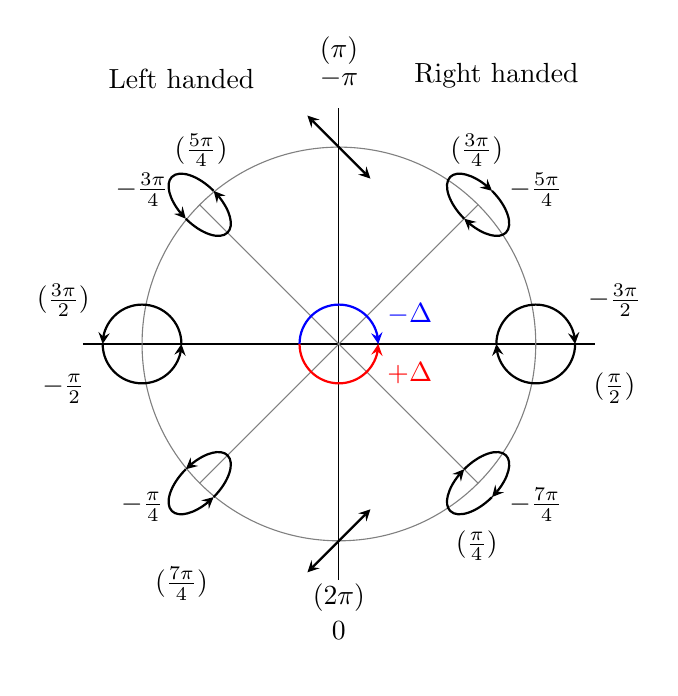
\begin{tikzpicture}
    
    % Axes
    \draw (-3.25,0)--(3.25,0);
    \draw (0,-3)--(0,3);
    \draw[thin, gray] (-1.77,-1.77)--(1.77,1.77);
    \draw[thin, gray] (1.77,-1.77)--(-1.77,1.77);
    
    \draw[thin, gray] (0,0) circle (2.5);
    
    % States
    \draw[<->, thick, >=stealth] (0.4,-2.1) -- (-0.4,-2.9);
    \draw[<->, thick, >=stealth] (0.4,2.1) -- (-0.4,2.9);
    
    \draw[-{>[flex=0.85]}, >=stealth, thick] (2,0) arc (180:0:0.5);
    \draw[-{>[flex=0.85]}, >=stealth, thick] (3,0) arc (0:-180:0.5);

    \draw[-{>[flex=0.85]}, >=stealth, thick] (-2,0) arc (0:180:0.5);
    \draw[-{>[flex=0.85]}, >=stealth, thick] (-3,0) arc (-180:0:0.5);
    
    % bot left 
    \draw [-{>[flex=0.85]}, thick, >=stealth, rotate=-45] (0.25,-2.5) arc [start angle=0, end angle=180, x radius=0.25, y radius=0.5];
    \draw [-{>[flex=0.85]}, thick, >=stealth, rotate=-45] (-0.25,-2.5) arc [start angle=-180, end angle=0, x radius=0.25, y radius=0.5];
    
    % top left
    \draw [-{>[flex=0.85]}, thick, >=stealth, rotate=45] (0.25,2.5) arc [start angle=0, end angle=180, x radius=0.25, y radius=0.5];
    \draw [-{>[flex=0.85]}, thick, >=stealth, rotate=45] (-0.25,2.5) arc [start angle=-180, end angle=0, x radius=0.25, y radius=0.5];
    
    % bot right
    \draw [-{>[flex=0.85]}, thick, >=stealth, rotate=-135] (0,2.75) arc [start angle=90, end angle=-90, x radius=0.5, y radius=0.25];
    \draw [-{>[flex=0.85]}, thick, >=stealth, rotate=-135] (0,2.25) arc [start angle=270, end angle=90, x radius=0.5, y radius=0.25];
    
    % top right
    \draw [-{>[flex=0.85]}, thick, >=stealth, rotate=-45] (0,2.75) arc [start angle=90, end angle=-90, x radius=0.5, y radius=0.25];
    \draw [-{>[flex=0.85]}, thick, >=stealth, rotate=-45] (0,2.25) arc [start angle=270, end angle=90, x radius=0.5, y radius=0.25];
    
    % inner circle
    \draw[-{>[flex=0.85]}, >=stealth, thick, blue] (-0.5,0) arc (180:0:0.5);
    \draw[-{>[flex=0.85]}, >=stealth, thick, red] (-0.5,0) arc (-180:0:0.5);
    
    % labels
    \draw (2, 3) node[label={[align=left] Right handed}] {};
    \draw (-2, 3) node[label={[align=left] Left handed}] {};
    
    \draw (0, 3.3) node[label={$(\pi)$}] {};
    \draw (0, 3.) node[label={$-\pi$}] {};
    
    \draw (0, -3.65) node[label={$(2\pi)$}] {};
    \draw (0, -4) node[label={$0$}] {};
    
    \draw (-2.5, -2.5) node[label={$-\frac{\pi}{4}$}] {};
    \draw (-2, -3.5) node[label={$(\frac{7\pi}{4})$}] {};
    
    \draw (-3.5, 0.1) node[label={$(\frac{3\pi}{2})$}] {};
    \draw (-3.5, -1) node[label={$-\frac{\pi}{2}$}] {};
    
    \draw (-1.75, 2) node[label={$(\frac{5\pi}{4})$}] {};
    \draw (-2.5, 1.5) node[label={$-\frac{3\pi}{4}$}] {};
    
    \draw (1.75, -3) node[label={$(\frac{\pi}{4})$}] {};
    \draw (2.5, -2.5) node[label={$-\frac{7\pi}{4}$}] {};
    
    \draw (1.75, 2) node[label={$(\frac{3\pi}{4})$}] {};
    \draw (2.5, 1.5) node[label={$-\frac{5\pi}{4}$}] {};
    
    \draw (3.5, 0.1) node[label={$-\frac{3\pi}{2}$}] {};
    \draw (3.5, -1) node[label={$(\frac{\pi}{2})$}] {};
    
    \draw[blue] (0.9, 0) node[label={$-\Delta$}] {};
    \draw[red] (0.9, -0.75) node[label={$+\Delta$}] {};
    
\end{tikzpicture}
\end{document}